
\section{Overview}

The framework has four stages. \textbf{Stage 0} transforms the observables into log
space using the power-law structure of accretion. \textbf{Stage 1} finds regime
boundaries with recursive binary segmentation, a lagged Chow $F$-test, and BIC.
\textbf{Stage 2} estimates a dynamic causal graph for each regime with DYNOTEARS.
\textbf{Stage 3} validates the resulting causal effects.

The physical states are introduced first in Figure~\ref{fig:section-c-1}. Their
hypothesised causal structures are then shown in Figure~\ref{fig:section-c-2}. The
complete recursive pipeline appears in Figure~\ref{fig:pipeline}.

\begin{figure}[htbp]
    \centering
    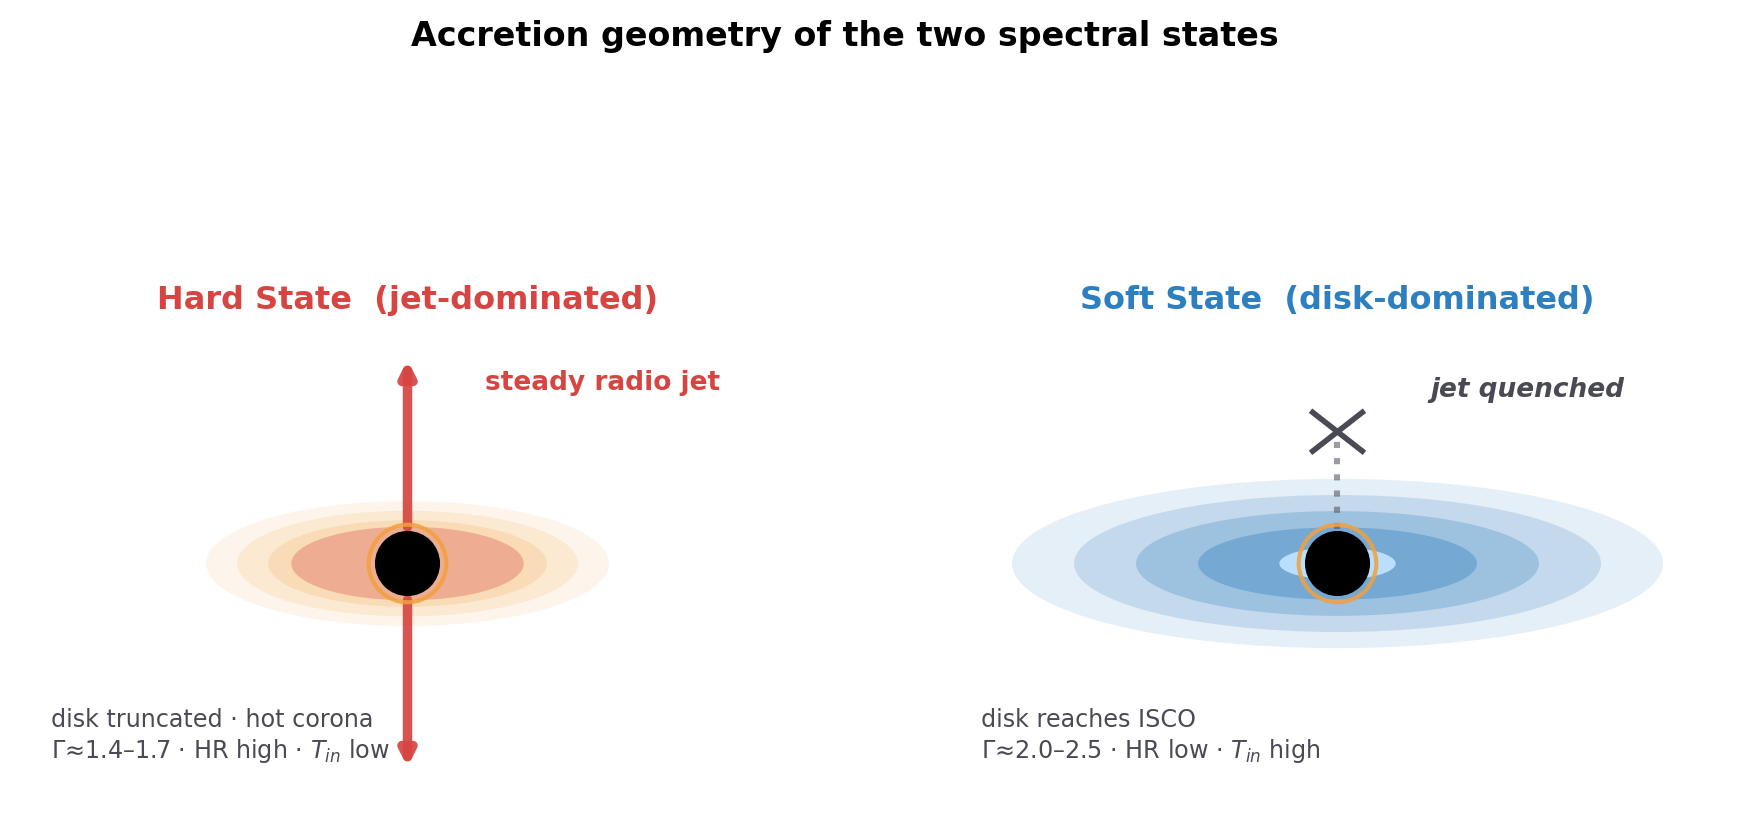
\includegraphics[width=\textwidth]{figs/fig01_accretion_states.png}
\caption{Accretion geometry of the two spectral states. In the Hard State the disk is truncated and replaced inward by a hot corona, with a steady radio jet. In the Soft State the disk extends to the innermost stable circular orbit and the jet is quenched.}
    \label{fig:section-c-1}
\end{figure}

Figure~\ref{fig:section-c-1} compares the two accretion states. In the Hard State,
the inner disk is truncated and replaced by a hot corona, while a steady radio jet
is present. In the Soft State, the disk extends to the innermost stable circular
orbit and the radio jet is quenched.



\begin{figure}[htbp]
    \centering
    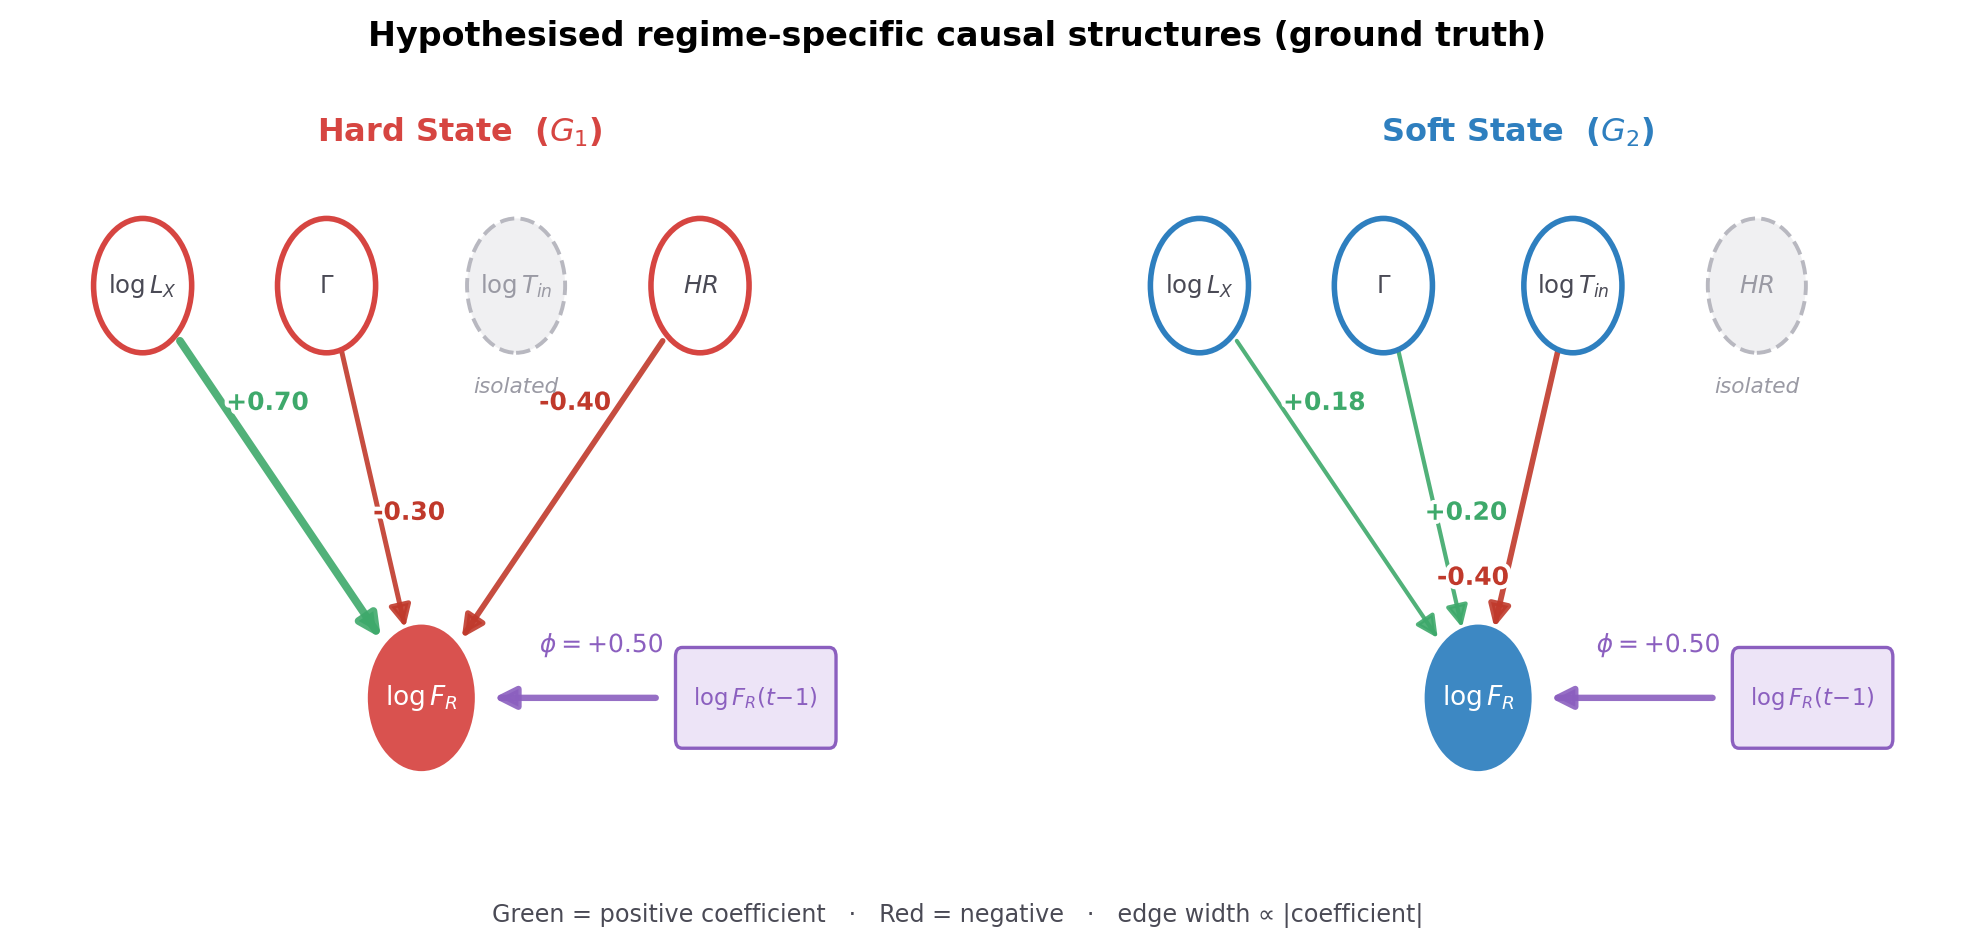
\includegraphics[width=\textwidth]{figs/fig02_ground_truth_dags.png}
\caption{Hypothesised causal structures for the hard and soft accretion states.}
    \label{fig:section-c-2}
\end{figure}

Figure~\ref{fig:section-c-2} shows the hypothesised causal structures for the two
states. The variables that influence radio luminosity differ between the Hard and
Soft States, and the isolated variable also changes. These regime-specific
structures motivate the graph-recovery stage of LIRA.

\begin{figure}[htbp]
    \centering
    \resizebox{\textwidth}{!}{%
    \begin{tikzpicture}[
        >=Stealth,
        node distance=8mm and 18mm,
        every node/.style={font=\small, align=center},
        process/.style={draw=gray!65!black, line width=0.5pt, rounded corners=2pt, minimum width=38mm, minimum height=9mm, text=black, fill=cyan!60},
        stage/.style={draw=gray!65!black, line width=0.5pt, rounded corners=2pt, minimum width=38mm, minimum height=9mm, text=black, fill=violet!50},
        gate/.style={draw=gray!65!black, line width=0.5pt, rounded corners=2pt, minimum width=38mm, minimum height=9mm, text=black, fill=orange!55},
        leaf/.style={draw=gray!65!black, line width=0.5pt, rounded corners=2pt, minimum width=38mm, minimum height=9mm, text=black, fill=gray!50},
        output/.style={draw=gray!65!black, line width=0.5pt, rounded corners=2pt, minimum width=38mm, minimum height=9mm, text=black, fill=teal!55},
        inputbox/.style={process, fill=green!60},
        olsbox/.style={stage, fill=violet!50},
        binbox/.style={stage, fill=blue!45},
        chowbox/.style={gate, fill=yellow!55},
        bicbox/.style={gate, fill=yellow!55},
        leafbox/.style={leaf, fill=gray!45},
        dynobox/.style={output, fill=pink!55},
        graphbox/.style={output, fill=brown!45},
        acceptbox/.style={process, fill=cyan!60},
        terminationbox/.style={leaf, fill=red!30},
        yes/.style={draw=gray!65!black, fill=green!15, rounded corners=2pt, inner sep=1.5pt, text=black, font=\bfseries\scriptsize},
        no/.style={draw=gray!65!black, fill=red!12, rounded corners=2pt, inner sep=1.5pt, text=black, font=\bfseries\scriptsize},
        line/.style={->, thick, draw=gray!60!black}
    ]
        \node[inputbox] (input) {\textbf{Node input}};
        \node[olsbox, below=of input] (ols) {\textbf{Fit lagged OLS}};
        \node[binbox, below=of ols] (binseg) {\textbf{Binary segmentation}};
        \node[chowbox, below=of binseg] (chow) {\textbf{Gate 1: Chow test}};
        \node[bicbox, below=of chow] (bic) {\textbf{Gate 2: BIC check}};
        \node[leafbox, below left=12mm and 24mm of bic] (leafnode) {\textbf{Declare leaf}};
        \node[dynobox, below=of leafnode] (dyno) {\textbf{Apply DYNOTEARS}};
        \node[graphbox, below=of dyno] (graph) {\textbf{Regime-specific causal graph}};
        \node[terminationbox, below=of graph] (stop) {\textbf{Termination}};
        \node[acceptbox, below right=12mm and 24mm of bic] (accept) {\textbf{Accept split}};

        \draw[line] (input) -- (ols);
        \draw[line] (ols) -- (binseg);
        \draw[line] (binseg) -- (chow);
        \draw[line] (chow) -- node[right, yes] {YES} (bic);
        \draw[line] (chow) -| node[above, no] {NO} (leafnode);
        \draw[line] (bic) -| node[above, no] {NO} (leafnode);
        \draw[line] (bic) -- node[right, yes] {YES} (accept);
        \draw[line] (leafnode) -- (dyno);
        \draw[line] (dyno) -- (graph);
        \draw[line] (graph) -- (stop);
        \draw[line] (accept.east) -- ++(15mm,0) |- (ols.east);
    \end{tikzpicture}%
    }
    \caption{Step-by-step recursive framework for temporal regime discovery and dynamic causal graph recovery, combining lagged OLS estimation, Binary Segmentation, Chow and BIC gates, and DYNOTEARS.}
    \label{fig:pipeline}
\end{figure}

Figure~\ref{fig:pipeline} summarises the complete procedure. The method fits a
lagged OLS model, searches for a candidate boundary with binary segmentation, and
passes it through the Chow and BIC gates. Accepted splits are processed recursively.
When a leaf is reached, DYNOTEARS estimates the regime-specific causal graph. The
validation results for this process are presented in Chapter 5.

\section{Log-space linearisation}

The Fundamental Plane of Black Hole Activity expresses radio luminosity as a power law
in X-ray luminosity and black hole mass, as shown in Equation~\eqref{eq:ch4-1}:

\begin{equation}
    \label{eq:ch4-1}
L_R \propto L_X^{\xi_X} \cdot M_{BH}^{\xi_M}
\end{equation}

Taking logarithms converts Equation~\eqref{eq:ch4-1} into coefficients and addition:

\begin{equation}
    \label{eq:ch4-2}
\log L_R = \xi_X \log L_X + \xi_M \log M_{BH} + c
\end{equation}

Equation~\eqref{eq:ch4-2} is linear. This form is required by OLS, the Chow test,
the $F$-distribution derivation, BIC, and the linear DYNOTEARS model. In raw flux
space the relationships would remain multiplicative, so these linear-model results
would not apply. The reasoning is summarised in Equation~\eqref{eq:ch4-3}:

\begin{equation}
    \label{eq:ch4-3}
\text{accretion physics} \Rightarrow \text{power laws} \Rightarrow \text{log-linearity} \Rightarrow \text{OLS valid} \Rightarrow \text{Chow and BIC valid}
\end{equation}

The log transform is derived from the physical scaling law rather than chosen only as
a generic preprocessing step.

Table~\ref{tab:ch4-variables} gives the transformation used for each variable.



\begin{table}[htbp]
    \centering
    \small
    \caption{Variable set and transformation}
    \label{tab:ch4-variables}
    \begin{tabularx}{\textwidth}{|>{\raggedright\arraybackslash}p{1.3cm}|>{\raggedright\arraybackslash}p{2.6cm}|>{\raggedright\arraybackslash}p{1.9cm}|>{\raggedright\arraybackslash}X|}
        \hline
        Symbol & Quantity & Transform & Justification \\ \hline
        $F_R$ & radio luminosity & $\log$ & Luminosity. Power-law coupled and spans orders of magnitude. \\ \hline
        $L_X$ & X-ray luminosity & $\log$ & Luminosity. Power-law coupled and spans orders of magnitude. \\ \hline
        $T_{in}$ & inner disk temperature & $\log$ & multicolor disk models give power-law scaling with luminosity \\ \hline
        $\Gamma$ & photon index & none & already a dimensionless spectral slope, itself an exponent. Range $\approx 1.4$--$2.5$ \\ \hline
        $HR$ & hardness ratio & none & already a bounded dimensionless ratio. The same argument applies as for $\Gamma$. \\ \hline
\end{tabularx}
\end{table}

The dimensionless, bounded variables $\Gamma$ and $HR$ are left unchanged. They do
not require logarithmic compression, and the power-law argument does not apply to
them.

The spectral-state diagnostics used by the model are summarised in Table~\ref{tab:ch4-states}.


\section{The structural model}


\subsection{Absorption of black hole mass}

Equation~\eqref{eq:ch4-2} contains $\log M_{BH}$. For a single accreting source observed over
time, $M_{BH}$ is constant: it cannot vary between time steps. A constant term in a
regression equation is absorbed entirely by the intercept, as shown in Equation~\eqref{eq:ch4-4}:

\begin{equation}
    \label{eq:ch4-4}
\xi_M \log M_{BH} \;\longrightarrow\; \text{folded into } w_0
\end{equation}

so mass is absorbed into the intercept. This is the correct treatment of a
within-source constant. LIRA's coefficients therefore describe variation within one
source and are not directly comparable to the cross-source Fundamental Plane
exponents.


\subsection{Spectral-state variables}

The model needs time-varying quantities to distinguish physical states. The standard
spectral-state diagnostics provide these variables, as summarised in
Table~\ref{tab:ch4-states}.



\begin{table}[htbp]
    \centering
    \small
    \caption{Spectral-state diagnostics and their regime dependence}
    \label{tab:ch4-states}
    \begin{tabularx}{\textwidth}{|>{\raggedright\arraybackslash}p{1.8cm}|>{\raggedright\arraybackslash}p{2.5cm}|>{\raggedright\arraybackslash}p{2.5cm}|>{\raggedright\arraybackslash}X|}
        \hline
        Variable & Hard State & Soft State & Physical quantity indexed \\ \hline
        $\log L_X$ & lower & higher & accretion rate \\ \hline
        $\Gamma$ & flat, $\approx1.4$--$1.7$ & steep, $\approx2.0$--$2.5$ & Comptonisation vs. disk emission \\ \hline
        $\log T_{in}$ & lower (disk truncated) & higher (disk at ISCO) & disk inner radius / geometry \\ \hline
        $HR$ & high & low & spectral hardness \\ \hline
\end{tabularx}
\end{table}

These variables do not replace mass. They capture temporal state variation within one
source, which the cross-source Fundamental Plane does not represent. The resulting
static specification is given in Equation~\eqref{eq:ch4-5}:

\begin{equation}
    \label{eq:ch4-5}
\log F_R(t) = w_0 + w_1 \log L_X(t) + w_2 \Gamma(t) + w_3 \log T_{in}(t) + w_4 HR(t) + \varepsilon(t)
\end{equation}


\subsection{The autoregressive extension}

The static specification in Equation~\eqref{eq:ch4-5} would require i.i.d. errors,
which real accretion time series do not satisfy. Time series show memory from viscous
timescales, turbulence, propagating
fluctuations, and persistent jets. The main consequences are:

\begin{enumerate}
    \item OLS coefficient estimates remain unbiased.
    \item Standard errors are underestimated.
    \item \textbf{The Chow $F$-statistic breaks.} Its denominator assumes i.i.d. residuals. Under
autocorrelation the denominator is artificially small, the $F$-statistic
artificially large, and the procedure detects regime boundaries that do not exist.
\end{enumerate}

The third consequence is the most important: unmodelled autocorrelation can create
false regime boundaries. We address it by adding the first-order autoregressive term
in Equation~\eqref{eq:ch4-6}:

\begin{equation}
    \label{eq:ch4-6}
\log F_R(t) = w_0 + w_1 \log L_X(t) + w_2 \Gamma(t) + w_3 \log T_{in}(t) + w_4 HR(t) + \phi \log F_R(t-1) + \varepsilon(t)
\end{equation}

Here, $\phi$ absorbs the temporal dependence, making $\varepsilon(t)$ approximately
i.i.d. and restoring the test assumptions. Section~5.2 verifies this result.

The coefficient $\phi$ measures temporal persistence and can be compared across
regimes (Section~5.4).

Lag one is used as the minimum sufficient choice. Additional lags increase $q$, reduce
the residual degrees of freedom, and make smaller regime segments harder to estimate.
If residual autocorrelation remains, Newey--West standard errors provide a robustness
check.


\subsection{Choice of estimator}

\textbf{Regularised regression is excluded.} Ridge and Lasso add penalties
($\lambda\|\beta\|_2^2$ and $\lambda\|\beta\|_1$ respectively) that shrink coefficients
toward zero, biasing the estimates. Since the Chow test consists entirely of comparing
the coefficient vectors of two groups, shrinking both corrupts the comparison: the test
would partly detect differences induced by the penalty rather than by genuine mechanism
change. Stage 1 therefore requires unbiased estimates and must not regularise.

This is deliberately in contrast with Stage 2, where DYNOTEARS does employ an $L_1$
penalty. The two stages answer different questions. Stage 2 asks \textit{which edges exist},
for which sparsity is essential. Stage 1 asks \textit{whether two coefficient vectors are
equal}, for which bias is fatal.

\textbf{Polynomial terms are excluded.} The log-linear form is derived from power-law
physics (Section~4.2). Terms such as $(\log L_X)^2$ have no physical motivation, invite
overfitting, and violate the assumption of common functional form across groups
required by the $F$-statistic derivation.


\subsection{Design matrix}

The design matrix has shape $(n-1, 6)$, the first observation being unavailable as a
response because it has no lag. Equations~\eqref{eq:ch4-7} and~\eqref{eq:ch4-8}
show the design matrix and response vector:

\begin{equation}
    \label{eq:ch4-7}
X_{lag} = \begin{bmatrix}
1 & \log L_X(2) & \Gamma(2) & \log T_{in}(2) & HR(2) & \log F_R(1) \\
1 & \log L_X(3) & \Gamma(3) & \log T_{in}(3) & HR(3) & \log F_R(2) \\
\vdots & \vdots & \vdots & \vdots & \vdots & \vdots \\
1 & \log L_X(n) & \Gamma(n) & \log T_{in}(n) & HR(n) & \log F_R(n-1)
\end{bmatrix}
\end{equation}

\begin{equation}
    \label{eq:ch4-8}
Y = [\log F_R(2), \log F_R(3), \ldots, \log F_R(n)]^\top
\end{equation}

With the OLS solution given by the normal equation in Equation~\eqref{eq:ch4-9},
Equation~\eqref{eq:ch4-10} gives the residuals and residual sum of squares:

\begin{equation}
    \label{eq:ch4-9}
\hat{w} = (X_{lag}^\top X_{lag})^{-1} X_{lag}^\top Y, \qquad \hat{w} = [w_0, w_1, w_2, w_3, w_4, \phi]^\top
\end{equation}

\begin{equation}
    \label{eq:ch4-10}
\hat{\varepsilon} = Y - X_{lag}\hat{w}, \qquad RSS_{global} = \hat{\varepsilon}^\top \hat{\varepsilon}
\end{equation}

$RSS_{global}$ measures how well a \textbf{single} causal model fits the entire series and
serves as the baseline against which all partitions are compared.


\section{Gate 1: the lagged Chow test}


\subsection{Hypothesis and intuition}

\begin{equation}
    \label{eq:ch4-11}
H_0 : w_A = w_B
\end{equation}

Equation~\eqref{eq:ch4-11} is the null hypothesis. Rejecting it indicates that the
mechanism differs between the two groups. If the two states follow different laws,
separate models should have lower residual error than one pooled model. The test
determines whether this reduction is statistically significant.

Note that $w$ includes the intercept $w_0$. This has a direct consequence for the
design of the validation data, addressed in Section~5.1.


\subsection{Construction}

For a candidate split, let $A$ denote observations before and $B$ after. Separate fits
are given in Equations~\eqref{eq:ch4-12} and~\eqref{eq:ch4-13}:

\begin{equation}
    \label{eq:ch4-12}
\hat{w}_A = (X_A^\top X_A)^{-1} X_A^\top Y_A, \quad RSS_A = \|Y_A - X_A\hat{w}_A\|^2
\end{equation}
\begin{equation}
    \label{eq:ch4-13}
\hat{w}_B = (X_B^\top X_B)^{-1} X_B^\top Y_B, \quad RSS_B = \|Y_B - X_B\hat{w}_B\|^2
\end{equation}

Equation~\eqref{eq:ch4-14} gives the Chow statistic. The cost of pooling is $RSS_{global} - (RSS_A + RSS_B)$, which is near zero when both
groups share one causal law. Normalising by the within-group variance
$\hat\sigma^2 = (RSS_A + RSS_B)/(n-2q)$ yields the lagged Chow statistic:

\begin{equation}
    \label{eq:ch4-14}
F_{lag} = \frac{\big[RSS_{global} - (RSS_A + RSS_B)\big] / q}{(RSS_A + RSS_B)/(n - 2q)}
\end{equation}

The numerator is divided by $q$ because the split adds $q$ parameters. The denominator
has $n-2q$ degrees of freedom, the residual degrees of freedom after fitting two
models.


\subsection{Degrees of freedom}

The value $q = 6$ follows directly from the structural model of Section~4.3 and is not a
tuning parameter: the intercept $w_0$ (which absorbs $\xi_M \log M_{BH}$), the four
spectral-state coefficients $w_1$--$w_4$, and the autoregressive coefficient $\phi$.


\subsection{Distribution}

Under $H_0$ and Gaussian i.i.d. residuals, Equation~\eqref{eq:ch4-15} gives the numerator and denominator distributions:
independent chi-square variates,

\begin{equation}
    \label{eq:ch4-15}
\big[RSS_{global} - (RSS_A + RSS_B)\big]/\sigma^2 \sim \chi^2(q), \qquad (RSS_A + RSS_B)/\sigma^2 \sim \chi^2(n-2q)
\end{equation}

and the ratio of two independent chi-square variables each divided by its degrees of
freedom is $F$-distributed by definition, as shown in Equation~\eqref{eq:ch4-16}:

\begin{equation}
    \label{eq:ch4-16}
F_{lag} \sim F(q,\; n-2q) \quad \text{under } H_0
\end{equation}

\begin{equation}
    \label{eq:ch4-17}
p = P\big(F(q, n-2q) > F_{obs}\big) = 1 - \mathrm{CDF}_F(F_{obs}, q, n-2q)
\end{equation}

$H_0$ is rejected at $\alpha=0.05$. The test requires Gaussian residuals, which also
constrains the downstream causal-discovery model. This issue is discussed in
Section~4.6.


\section{Locating the boundary and Gate 2}


\subsection{Binary segmentation}

The test of Section~4.4 requires a split point to be supplied. Since the boundary location is
unknown, the statistic is evaluated at every admissible index and maximised, as shown
in Equation~\eqref{eq:ch4-18}:

\begin{equation}
    \label{eq:ch4-18}
\tau^* = \arg\max_{\tau} F_{lag}\big(A(\tau), B(\tau)\big)
\end{equation}

where $A(\tau) = \{2,\ldots,\tau\}$ and $B(\tau) = \{\tau+1,\ldots,n\}$. The maximising
index is the location at which the data most strongly prefers two models to one.

Exhaustive search over all multi-way partitions is intractable. Binary segmentation
is therefore used as a greedy divide-and-conquer method: it finds the best split and
then repeats the search within each child segment. This procedure is not guaranteed
to find the global optimum.

A minimum segment size of $2q=12$ is enforced. Smaller segments do not support
stable matrix inversion, and the $F$-test degrees of freedom approach zero. Segments
near this minimum can still produce noisy coefficients and unreliable graphs.

\textbf{Note on splitting variable.} Splitting is performed on the time index only.
Feature-threshold splitting of the form $(j^*, \tau^*)$ is not employed, as the
autoregressive term of (4.5) presupposes temporal contiguity within each segment.


\subsection{Derivation of the BIC criterion}

A significant $F$-statistic shows that a difference is detectable, but a greedy search
can find apparently favourable splits caused by noise. Without a stopping rule, the
algorithm would continue splitting until the segments became too small. BIC provides
the required complexity penalty.

\textbf{Step A: the Gaussian likelihood.} For $Y = Xw + \varepsilon$ with
$\varepsilon_t \sim N(0,\sigma^2)$ i.i.d., Equation~\eqref{eq:ch4-19} gives the Gaussian likelihood.

\begin{equation}
    \label{eq:ch4-19}
\log P(Y \mid w, \sigma^2, M) = -\frac{n}{2}\log(2\pi) - \frac{n}{2}\log(\sigma^2) - \frac{RSS}{2\sigma^2}
\end{equation}

\textbf{Step B: substitution of the MLE.} With $\hat\sigma^2 = RSS/n$, Equation~\eqref{eq:ch4-20} gives the likelihood at the MLE.

\begin{equation}
    \label{eq:ch4-20}
\log P(Y \mid \hat{w}, \hat\sigma^2, M) = -\frac{n}{2}\log(2\pi) - \frac{n}{2}\log\!\left(\frac{RSS}{n}\right) - \frac{n}{2}
\end{equation}

The terms $-\frac{n}{2}\log(2\pi)$ and $-\frac{n}{2}$ do not depend on the model and
cancel in any comparison, leaving the simplified likelihood in Equation~\eqref{eq:ch4-21}:

\begin{equation}
    \label{eq:ch4-21}
\log P \approx -\frac{n}{2}\log\!\left(\frac{RSS}{n}\right)
\end{equation}

\textbf{Step C: the criterion.} Schwarz's criterion, obtained from the Laplace
approximation to the marginal likelihood, is $BIC = -2\log P(Y \mid \hat\theta, M) + k\log(n)$
for $k$ free parameters. Substituting Equation~\eqref{eq:ch4-19}, we obtain the BIC
given in Equation~\eqref{eq:ch4-22}:

\begin{equation}
    \label{eq:ch4-22}
BIC = n\log\!\left(\frac{RSS}{n}\right) + k\log(n)
\end{equation}

\textbf{Step D: the one-model case.} For a single global model over $n$ observations with
$q = 6$ parameters, Equation~\eqref{eq:ch4-23} gives the one-model BIC:

\begin{equation}
    \label{eq:ch4-23}
BIC_1 = n\log\!\left(\frac{RSS_{global}}{n}\right) + q\log(n)
\end{equation}

\textbf{Step E: the two-model case.} For disjoint segments the combined log-likelihood is
the sum of the two independent log-likelihoods, each with its own MLE
$\hat\sigma_A^2 = RSS_A/n_A$ and $\hat\sigma_B^2 = RSS_B/n_B$. With $2q$ total free
parameters, as shown in Equation~\eqref{eq:ch4-24}:

\begin{equation}
    \label{eq:ch4-24}
BIC_2 = n_A\log\!\left(\frac{RSS_A}{n_A}\right) + n_B\log\!\left(\frac{RSS_B}{n_B}\right) + 2q\log(n)
\end{equation}

\textbf{Step F: the choice of $\log(n)$.} The penalty uses the total sample size $n$,
following the Bai--Perron convention for structural-break models. Using $n_A$ and
$n_B$ separately would make small segments cheaper and encourage over-partitioning.
Using total $n$ keeps the two scores on a common scale.

\textbf{Step G: decision rule.} A split is accepted if and only if $BIC_2 < BIC_1$.
Subtracting the penalty of Equation~\eqref{eq:ch4-23} from the penalty of
Equation~\eqref{eq:ch4-24} gives the net penalty
increase from splitting, as shown in Equation~\eqref{eq:ch4-25}:

\begin{equation}
    \label{eq:ch4-25}
2q\log(n) - q\log(n) = q\log(n)
\end{equation}

which is the exact price, in units of $-2\log$-likelihood, of admitting one additional
regime.


\subsection{Why BIC rather than AIC}

AIC imposes a penalty of $2k$, constant in sample size. BIC imposes $k\log(n)$, which
grows with the data. Table~\ref{tab:ch4-bic} gives the comparison at $k = q = 6$.



\begin{table}[htbp]
    \centering
    \small
    \caption{Complexity penalty comparison}
    \label{tab:ch4-bic}
    \begin{tabularx}{\textwidth}{|X|X|X|X|}
        \hline
        $n$ & AIC penalty & BIC penalty & Ratio \\ \hline
        800 & 12 & 40.1 & 3.3$\times$ \\ \hline
        5,000 & 12 & 51.1 & 4.3$\times$ \\ \hline
        10,000 & 12 & 55.3 & 4.6$\times$ \\ \hline
\end{tabularx}
\end{table}

For regime discovery, a false split can corrupt both resulting graphs, while a missed
split gives a conservative pooled model. BIC's stronger, sample-size-dependent
penalty is therefore appropriate for this task.


\subsection{The two-gate design}

The two criteria serve different purposes. The Chow test asks whether the difference
is statistically detectable. BIC asks whether the improvement justifies the added
complexity. A split can pass the first test and fail the second, as shown in Section~5.3.


\section{Identifiability}

For a linear structural equation model with Gaussian noise, edge direction within a
\textit{chain} ($X \to Y \to Z$) or \textit{fork} ($X \leftarrow Y \to Z$) is not identifiable from
observational data: for any true $X \to Y$ there exists a reversed model with rescaled
coefficient and noise variance inducing an identical joint distribution. No algorithm
can recover the direction, as the information is absent from the data.

A \textit{collider}, several mutually independent parents converging on a common effect, is
the exception. Collider orientation is recoverable from conditional-independence
structure alone, irrespective of noise distribution. This is the v-structure argument
on which constraint-based discovery rests generally.

\textbf{The model of Section~4.3 is a collider.} $\log L_X$, $\Gamma$, $\log T_{in}$, and $HR$ are
specified as parents of $\log F_R$ and not of one another. Direction is therefore
identifiable here for structural reasons rather than incidentally.

This has a consequence for possible extensions that is worth stating explicitly.
Suppose the model were enriched with causal chains among the spectral variables. Those
edges would be chains and forks, and recovering their orientation would require
non-Gaussian innovations together with a LiNGAM-family estimator. However, the
$F$-distribution result (4.14) requires Gaussian residuals for the numerator and
denominator to be independent chi-square variates, and the BIC derivation (4.17)--(4.20)
begins from the Gaussian log-likelihood. Adopting non-Gaussian noise to secure
identifiability in Stage 2 would therefore weaken the distributional derivations
underpinning both gates of Stage 1. The collider specification avoids this tension:
Gaussian noise is retained, (4.14) and (4.20) hold exactly as derived, and Stage 2
orientations remain identifiable. The restriction to a collider structure is thus a
defended design decision rather than a simplifying convenience.


\section{Stage 2: regime-specific causal graphs}

Each leaf is a temporally contiguous segment treated as a stable causal regime, and
DYNOTEARS is applied independently within each. Two matrices are estimated
simultaneously: $W$, in which $W_{ij} \neq 0$ indicates that variable $j$ affects
variable $i$ within the same time step, and $A$, in which $A_{ij} \neq 0$ indicates
that variable $j$ at $t-1$ affects variable $i$ at $t$. Acyclicity of the
contemporaneous graph is enforced by the smooth algebraic constraint
$\mathrm{tr}(e^{W \circ W}) - d = 0$, replacing combinatorial search with
gradient-based optimisation.

DYNOTEARS is preferred to the PC algorithm on two grounds. The first, noted in Section~2.1.6,
is that PC returns a skeleton and partial orientation without edge weights and
requires a number of conditional independence tests that grows sharply once lagged
variables are admitted. The second is decisive in practice: the Fisher-Z test assumes
independent samples, an assumption violated outright by consecutive observations of an
autoregressive process with $\phi \approx 0.9$. Applied to such data, the test's null
distribution is misspecified, and in preliminary experiments this produced orientations
into variables that have no parents by construction.

Two implementation requirements are recorded. First, variables must be standardised
within each leaf before fitting, as the DYNOTEARS objective and its sparsity threshold
are scale-sensitive. Without standardisation, edges belonging to lower-variance
variables are systematically underweighted and may be eliminated by the $L_1$ penalty.
Second, the terminality of $F_R$ must be encoded as explicit per-edge exclusions
forbidding $F_R$ at any lag from being a parent of $L_X$, $\Gamma$, $T_{in}$, or $HR$.
A blanket node-level prohibition also suppresses the edge $F_R(t-1) \to F_R(t)$, which
the model of (4.5) explicitly requires.


\section{Stage 3: causal effect estimation and validation}

Stages 1 and 2 yield a graph. Stage 3 quantifies the effects it encodes and assesses
how far those quantities should be trusted.

For each discovered parent of $F_R$ within each regime, the causal effect is estimated
by backdoor adjustment, conditioning on the remaining parents. Unpenalised regression
is used here, for the reason given in Section~4.3.4: with the structure already determined,
regularisation contributes only bias. The lag term $\log F_R(t-1)$ must be included in
every adjustment set, since the predictors are autocorrelated with their own past and
$F_R(t-1)$ lies downstream of that past. Omitting it allows a predictor to absorb part
of the lag term's effect.

Three refutation procedures are applied. A \textbf{random common cause} test injects an
irrelevant synthetic covariate, under which a valid estimate should be unchanged. A
\textbf{placebo treatment} test replaces the treatment with a permuted version, under which
the estimated effect should collapse to zero. This is the diagnostic that would expose
a procedure generating effects from noise. A \textbf{data subset} test re-estimates on an
80% subsample, guarding against dependence on particular observations.

\textbf{Sensitivity analysis} is then applied in the partial-$R^2$ parameterisation of
Cinelli and Hazlett, which reports a \textit{robustness value}: the minimum proportion of
residual variance in both treatment and outcome that an unobserved confounder would
need to explain in order to reduce the estimate to zero. Unobserved confounding cannot
be excluded from observational data, and Section~1.6 identifies it as a principal challenge
for this application. The robustness value converts that acknowledged limitation into
a stated numerical threshold against which domain knowledge can be brought to bear.

Finally, \textbf{graph falsification} tests whether the conditional-independence
implications of the entire recovered DAG are consistent with the data, by comparing
its violation count against randomly permuted graphs. Where the preceding tests
validate individual effects conditional on the graph, this interrogates the graph
itself.


\section{Parameter summary}

The complete parameter specification is given in Table~\ref{tab:ch4-parameters}.



\begin{table}[htbp]
    \centering
    \small
    \caption{Complete parameter specification}
    \label{tab:ch4-parameters}
    \begin{tabularx}{\textwidth}{|>{\raggedright\arraybackslash}X|>{\raggedright\arraybackslash}p{1.7cm}|>{\raggedright\arraybackslash}X|}
        \hline
        Parameter & Value & Determined by \\ \hline
        Variables log-transformed & $F_R, L_X, T_{in}$ & power-law scaling (Section~4.2) \\ \hline
        Variables untransformed & $\Gamma, HR$ & dimensionless, bounded range (Section~4.2) \\ \hline
        $q$ (parameters per model) & 6 & structural model: $w_0$, $w_1$--$w_4$, $\phi$ (Section~4.4.3) \\ \hline
        Chow numerator d.f. & $q = 6$ & parameters gained by splitting (Section~4.4.2) \\ \hline
        Chow denominator d.f. & $n - 2q$ & residual d.f. after two fits (Section~4.4.2) \\ \hline
        $\alpha$ & 0.05 & conventional; asymmetric error cost handled by Gate 2 \\ \hline
        $BIC$ penalty, one model & $q\log(n)$ & Schwarz criterion (Section~4.5.2) \\ \hline
        $BIC$ penalty, two models & $2q\log(n)$ & Bai--Perron convention, total $n$ (Section~4.5.2) \\ \hline
        Net cost of a split & $q\log(n)$ & Eq. (4.25) \\ \hline
        Lag order & 1 & minimum sufficient; higher orders raise $q$ (Section~4.3.3) \\ \hline
        Minimum segment size & $2q = 12$ & invertibility and $F$-test stability (Section~4.5.1) \\ \hline
        Splitting variable & time index & required by AR term (Section~4.5.1) \\ \hline
\end{tabularx}
\end{table}


